\section{LoraWAN}

LoRaWAN is a low-power, wide-area network protocol designed for IoT applications. 
It operates on a cellular-like architecture but is association-less, meaning devices do not need to establish permanent connections with the network. 
The main components of LoRaWAN include end devices, gateways, and a network server.

End devices are typically the field devices that generate data. 
Gateways serve as intermediaries, receiving messages from the end devices and forwarding them to the network server. 
The network server is the central hub where most of the intelligence of the system resides.
It is responsible for removing duplicate messages, managing acknowledgments, adjusting radio link parameters, and other essential tasks that ensure efficient communication.

\begin{figure}[H]
    \centering
    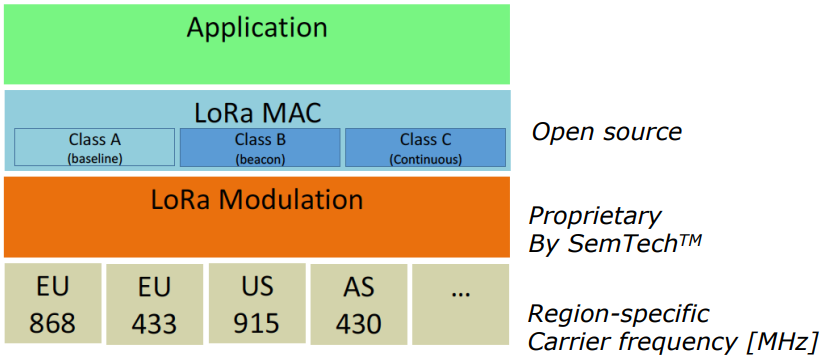
\includegraphics[width=0.5\linewidth]{images/lora.png}
    \caption{LoraWAN protocol stack}
\end{figure}

\paragraph*{Modulation}
The LoRaTM modulation scheme is based on a proprietary chirp-based spread spectrum technique. 
This method involves modulating a signal onto a chirp signal at a higher data rate. 
The chip rate (in chips per second) and nominal bit rate (in bits per second) are related by the formulas:
\[R_C=\text{BW}\qquad R_b=\text{SF}\dfrac{4\text{BW}}{2^{\text{SF}}(4+\text{CR})}\]
Here, $\text{BW}$ is the reference bandwidth, $\text{SF}$ is the spreading factor, and $\text{CR}$ is the coding rate. 

LoRaWAN balances two primary objectives: rate and reliability. 
The rate refers to how fast data can be transmitted, and reliability refers to how secure and stable the transmission is. 
For a given emitted power level, increasing the spreading factor improves sensitivity and reliability, while reducing SF increases the rate.
In general:
\begin{itemize}
    \item Lower spreading factors (SF) allow higher data rates.
    \item Higher spreading factors (SF) enhance reliability.
\end{itemize}
\noindent The minimum power level required for a given signal sensitivity is calculated by the formula:
\[P_{\min}=-174+10\log_{10}\text{BW}+\text{NF}+\text{SNR}\]
Here, $\text{BW}$ is the reference bandwidth, $\text{NF}$ is the noise figure, and $\text{SNR}$ is the signal-to-noise ratio. 

\paragraph*{End devices}
LoRaWAN defines three classes of end devices, each with different characteristics for handling downlink communications:
\begin{itemize}
    \item \textit{Class A}: this class allows for downlink messages to be received in slots that occur after the uplink transmission. 
        It uses an ALOHA-like access method for uplink communication, where devices randomly transmit messages when required.
    \item \textit{Class B}: in addition to the standard downlink slots, Class B devices have extra downlink slots that are scheduled at specific times, providing more predictable communication.
    \item \textit{Class C}: almost continuously listen for downlink messages, making them the most responsive but also the highest in power consumption.
\end{itemize}

\paragraph*{LoraWAN A}
In the European Union, the timing for receive windows in LoRaWAN Class A devices is standardized. 
If a preamble is detected during one of these receive windows, the radio receiver remains active until the downlink frame is demodulated. 
If a frame is detected and successfully demodulated during the first receive window, and the frame is intended for the end device (after address and Message Integrity Code checks), the device will not open the second receive window.
This method ensures energy efficiency, as the device only stays awake when necessary to receive messages, and it does not waste energy on unnecessary communication attempts.

\subsection{Messages}
LoRaWAN messages are structured in multiple layers that serve distinct functions for communication and integrity verification. 
\begin{figure}[H]
    \centering
    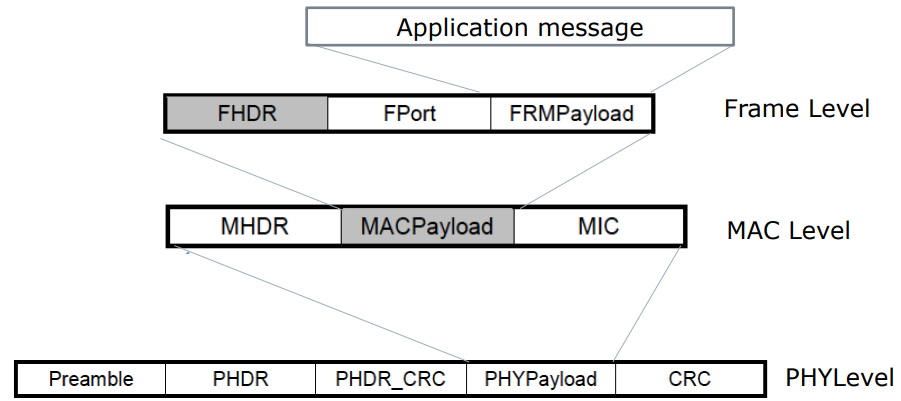
\includegraphics[width=0.5\linewidth]{images/lora1.png}
    \caption{LoraWAN messages}
\end{figure}
In particular, we have: 
\begin{itemize}
    \item \textit{PHY Message structure}: begins with the Preamble, a sequence of bits used to synchronize the transmitter and receiver.
        Following the preamble, the Physical Header contains essential information regarding the message, such as its type and format. 
        The PHDR\_CRC and CRC fields are used to perform integrity checks, ensuring that the message hasn't been corrupted during transmission. 
        The PHY Payload contains the actual data being sent in the message, or the payload, which varies depending on the type of communication.
    \item \textit{MAC Message Header}: specifies certain parameters about the message itself. 
        The MType field indicates the type of message being sent, distinguishing between various message types such as join requests or data uplinks. 
        The RFU (Reserved for Future Use) field is there to ensure future compatibility as the protocol evolves. 
        The Major field tells the receiver which message format is being used, making it possible for devices to communicate across different versions of the protocol.
    \item \textit{MAC message payload}: follows the header and is where the end device-related information is stored. 
        This section includes the DevAddr, a unique identifier assigned to the end device, ensuring that the message is directed to the correct device. 
        The FCtrl, or frame control field, is used to manage important features like adaptive data rate (ADR), acknowledgments (ACK), and MAC commands. 
        The FCnt is a counter that increments with each transmitted frame, ensuring proper sequencing of messages. 
        The FOpts field contains additional frame options, often used for sending MAC commands that control device behavior or optimize network resources.
    \item \textit{Frame Control Field}: critical part of the message, managing the transmission characteristics of the data.
        For example, the ADR (Adaptive Data Rate) function is used to optimize both the uplink and downlink data rates based on current network conditions, while the ADRACKReq flag requests an acknowledgment for ADR-related operations. 
        The ACK field acknowledges the successful reception of a message, confirming reliable communication.
        The FPending field signals whether there are additional frames waiting to be sent to the device in a downlink message. 
        Finally, the FOptsLen indicates the size of the FOpts field, allowing the receiver to interpret the data correctly.
\end{itemize}

\subsection{LoraWAN uplink}
LoRaWAN employs an ALOHA-like procedure to handle channel access and retransmissions. 
In this system, when a confirmed message is sent, if no acknowledgment (ACK) is received, the message is retransmitted after a random timeout. 
The timeout, referred to as ACK\_TIMEOUT, is randomly chosen from a time interval between 1 and 3 seconds and begins once Receive\_window2 concludes.

The ALOHA protocol does not require channel feedback; instead, it relies on the ACK to confirm receipt of the transmitted message. 
Time flows continuously within this protocol. 
When a message is ready for transmission, the first packet in the transmission queue is sent immediately. 
If an acknowledgment is not received, the message is retransmitted after a random delay, which corresponds to a randomly determined number of time slots.

In terms of performance, several assumptions are made for modeling the system. 
The assumption of stationarity means that the incoming and outgoing traffic rates, denoted as $S_{\text{in}}$ and $S_{\text{out}}$, are equal.
Traffic is distributed according to a Poisson process, with packet arrivals occurring randomly and independently over time.
The packet arrival rate is denoted by $\lambda$, and the transmission duration is represented by $T$. 
This leads to the definition of $G$ , which represents the total traffic on the channel and is calculated as $G=\lambda T$. 

The probability of successful transmission $\Pr_s$  is the likelihood that no other packet begins transmission during the conflict period of $2T$. 
This can be expressed as:
\[\Pr_s=\Pr(N(t-T,t+T)=0)=e^{-2G}\]
The throughput of the system, which refers to the successful transmissions per unit of time, is given by:
\[S=\text{GP}_s=Ge^{-2G}\]
This equation highlights the relationship between traffic load $G$ and the resulting throughput, showing that there is an optimal load for maximum throughput.